\chapter{Robotic arm Kinematic Analysis}


\section{Robotic arm, DH parameters \& Forward Kinematics}

The Forward Kinematics problem seeks to specify the way in which the robot's links are connected together. In other wants, we want to specify 
the transformations between every pair of consecutive robot links. It is known that the forward kinematics of a robot can be calculated given only four 
parameters for each link. These parameters are known in robotics as the \textbf{Denavit-Hartenberg} (DH) parameters. Two of these parameters describe the link 
itself and the other two describe the link's relation to the neighboring link.

\begin{itemize}
\item The \textbf{length} $L_i$ of the i-th link is equal to the distance between the axes $z_i$ and $z_{i+1}$
\item The \textbf{twist angle} $α_i$ of the i-th link, is the angle between the axes $z_i$ and $z_{i+1}$
\item The \textbf{rotation angle} $θ_i$ of the link $\left\lbrace i \right\rbrace $ with respect to the $\left\lbrace i-1 \right\rbrace$ link, is the angle 
between the axes $x_{i-1}$ and $x_i$
\item The \textbf{distance} $d_i$ of the link $\left\lbrace i \right\rbrace$ with respect to the $\left\lbrace i-1 \right\rbrace$ link, is the distance 
between the axes $x_{i-1}$ and $x_i$
\end{itemize}

\begin{center}
\begin{figure}[!htb]
\centering
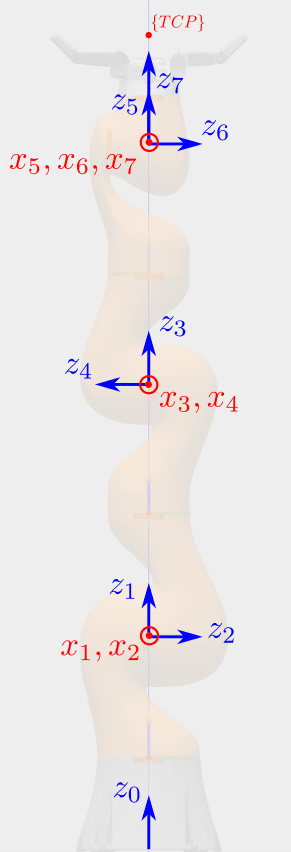
\includegraphics[height=12cm]{images/iiwa-frames.png}\\
\caption{Joint reference frames of the KUKA iiwa14 robot}
\end{figure}
\end{center}

\begin{center}
\begin{tabular}{ |c|c|c|c|c| } 
\hline
i & $θ_i$ (rad) & $L_{i-1}$ (m) & $d_i$ (m) & $α_{i-1}$ (rad) \\
\hline
1 & $θ_1$ & 0 & 0.36 & 0 \\
2 & $θ_2$ & 0 & 0 & $-π/2$ \\
3 & $θ_3$ & 0 & 0.36 & $π/2$ \\
4 & $θ_4$ & 0 & 0 & $π/2$\\
5 & $θ_5$ & 0 & 0.4 & $-π/2$ \\
6 & $θ_6$ & 0 & 0 & $-π/2$ \\
7 & $θ_7$ & 0 & 0 & $π/2$ \\
\hline
\end{tabular}
\end{center}

The goal of the forward kinematics problem is to find the transformation of the reference frame of the end-effector with respect to the universal reference frame. To achieve that, we must first calculate the 
transformations between each pair of joints. To simplify each such transformation, i.e. the transformation from a frame $\left\lbrace i-1 \right\rbrace$ to a frame $\left\lbrace i \right\rbrace$, we 
consider 3 intermediary reference frames $\left\lbrace A \right\rbrace$, $\left\lbrace B \right\rbrace$ and $\left\lbrace C \right\rbrace$. Then the transformations between the two joints is given by
\begin{equation}
^{i-1}T_i = ^{i-1}T_C \cdot ^{C}T_B \cdot ^{B}T_A \cdot ^{A}T_i
\end{equation}

The matrix $^{A}T_i$ expresses the translation of the coordinate system $\left\lbrace i \right\rbrace$ with respect to $\left\lbrace A \right\rbrace$ by a distance $d_i$ along the axis $z_i$
\begin{equation}
^{A}T_i = 
\begin{bmatrix}
1 & 0 & 0 & 0\\
0 & 1 & 0 & 0\\
0 & 0 & 1 & d_i\\
0 & 0 & 0 & 1\\
\end{bmatrix}
\end{equation}

The matrix $^{B}T_A$ expresses the rotation of the coordinate system $\left\lbrace A \right\rbrace$ with respect to $\left\lbrace B \right\rbrace$ by an angle $θ_i$ around the axis $z_i$
\begin{equation}
^{B}T_A = 
\begin{bmatrix}
c\theta_i & -s\theta_i & 0 & 0\\
s\theta_i & c\theta_i & 0 & 0\\
0 & 0 & 1 & 0\\
0 & 0 & 0 & 1\\
\end{bmatrix}
\end{equation}

The matrix $^{C}T_B$ expresses the translation of the coordinate system $\left\lbrace B \right\rbrace$ with respect to $\left\lbrace C \right\rbrace$ by a distance $L_{i-1}$ along the axis $x_{i-1}$
\begin{equation}
^{C}T_B = 
\begin{bmatrix}
1 & 0 & 0 & L_{i-1}\\
0 & 1 & 0 & 0\\
0 & 0 & 1 & 0\\
0 & 0 & 0 & 1\\
\end{bmatrix}
\end{equation}

The matrix $^{i-1}T_C$ expresses the rotation of the coordinate system $\left\lbrace C \right\rbrace$ with respect to $\left\lbrace i-1 \right\rbrace$ by an angle $a_{i-1}$ around the axis $x_{i-1}$
\begin{equation}
^{i-1}T_C = 
\begin{bmatrix}
1 & 0 & 0 & L_{i-1}\\
0 & ca_{i-1} & -sa_{i-1} & 0\\
0 & sa_{i-1} & ca_{i-1} & 0\\
0 & 0 & 0 & 1\\
\end{bmatrix}
\end{equation}

Using the DH parameters of the above table and the product of the above 4 matrices, one can calculate the transformation matrix between two consecutive links, and is calculated as the following

\begin{equation}
^{i-1}T_i = 
\begin{bmatrix}
c\theta_i & -s\theta_i & 0 & L_{i-1} \\
s\theta_ica_{i-1} & c\theta_ica_{i-1} & -sa_{i-1} & -sa_{i-1}d_i \\
s\theta_isa_{i-1} & c\theta_isa_{i-1} & ca_{i-1} & ca_{i-1}d_i \\
0 & 0 & 0 & 1\\
\end{bmatrix}
\end{equation}

When all the neighboring transformations are calculated, then one can calculate the total transformation $^{0}T_N$, which represents the position and the 
orientation of the local coordinate system of the end-effector with respect to the global coordinate system of the robot's base. The orientation is the 
upper-left 3x3 matrix and the position is given by the fourth column of the matrix $^{0}T_N$.

\begin{equation}
^{0}T_N = {}^{0}T_1 \cdot {}^{1}T_0 \cdots {}^{N-1}T_N
\end{equation}

All transformations $^{i-1}T_i$ are members of a special set of matrices (Lie Group), called \textbf{Special Euclidean Group}
\[
^{i-1}T_i \in SE(3) = \left\lbrace \begin{bmatrix}
R & \mathbf{p}\\
\mathbf{0} & 1
\end{bmatrix} : R \in SO(3), \mathbf{p} \in \mathbb{R}^{3} \right\rbrace
\]
where $SO(3)$ is another Lie Group called \textbf{Special Orthogonal Group}
\[
SO(3) = \left\lbrace R \in \mathbb{R}^{3 \times 3}: R^{-1}=R^\top, det(R)=1 \right\rbrace
\]

The properties of $SE(3)$ and $SO(3)$ are very useful in all the calculations of various transformations because it can reduce the amount of matrix operations and also speeds up the calculation 
of inverse matrices.

\begin{center}
\begin{figure}[!htb]
\centering
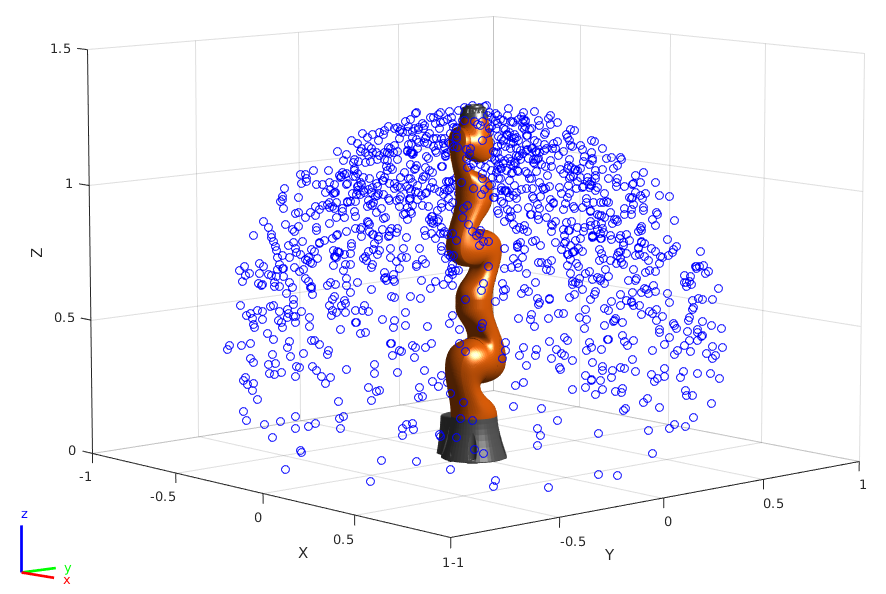
\includegraphics[width=0.5\textwidth]{images/workspace_sampling_1e3.png}\\
\caption{Approximation of the KUKA iiwa14 workspace, calculated with Forward Kinematics by randomly sampling the value ranges of the joints.}
\end{figure}
\end{center}

\subsection{End-effector to tool-tip transformations}

\begin{center}
\begin{figure}[!htb]
\centering
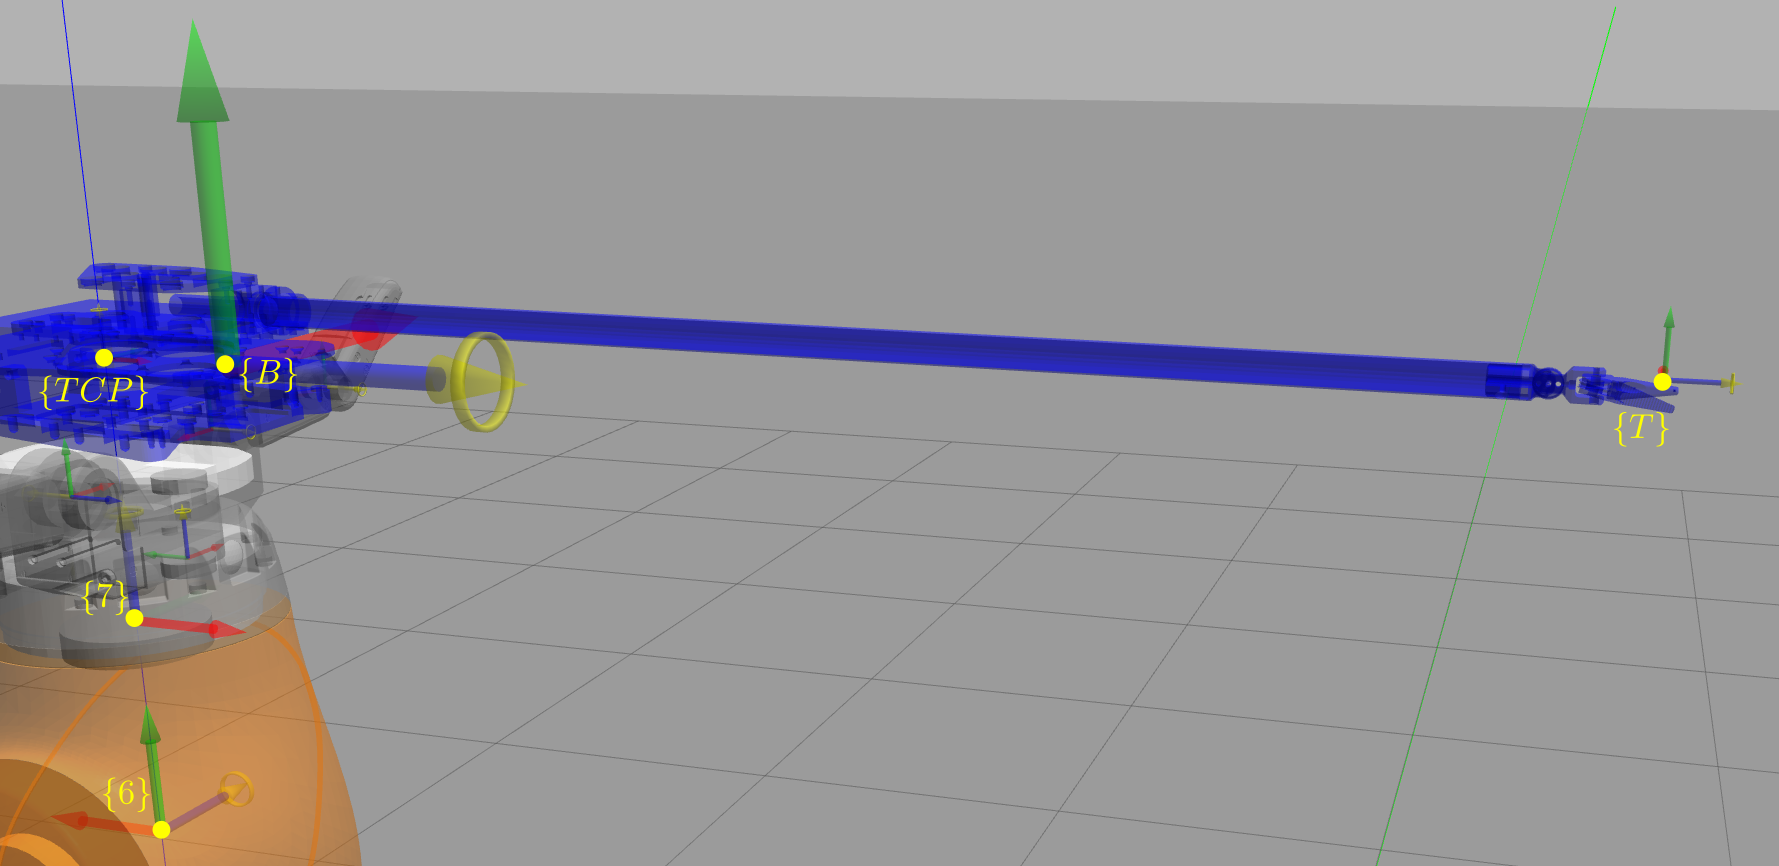
\includegraphics[width=\textwidth]{images/eef_tcp_tip_tf.png}\\
\caption{Reference frames of last link $\lbrace 7 \rbrace$, end-effector $\lbrace TCP \rbrace$, surgical tool base (center of mass) $\lbrace B \rbrace$ and tool-tip frame $\lbrace T \rbrace$}
\end{figure}
\end{center}

\[
^{7}T_{TCP} = 
\begin{bmatrix}
1 & 0 & 0 & 0 \\
0 & 1 & 0 & 0 \\
0 & 0 & 1 & 0.094 \\
0 & 0 & 0 & 1 \\
\end{bmatrix}
\]

\[
^{TCP}T_{B} = 
\begin{bmatrix}
1 & 0 & 0 & 0.05 \\
0 & 0 & -1 & 0 \\
0 & 1 & 0 & 0 \\
0 & 0 & 0 & 1 \\
\end{bmatrix}
\]

\[
^{B}T_T = 
\begin{bmatrix}
1 & 0 & 0 & -0.01 \\
0 & 1 & 0 & 0.022 \\
0 & 0 & 1 & 0.455 \\
0 & 0 & 0 & 1 \\
\end{bmatrix}
\]


\section{Inverse Kinematics}

The Inverse Kinematics problem is one of the most important problems a roboticist must solve to design trajectories and control the robot's motion to do useful tasks. The IK problem seeks to find 
those joint values that make the robot's end effector to be at a specific desired position and orientation or equivalently the input to this problem is the desired pose (position and orientation of the end-effector) 
and the output are the solutions for the joints. For a robot of six degrees of freedom, i.e. six actuators that move independently and are positioned in such a way so that their axes are not aligned, the solutions 
to the I.K. problem are typically 8. For robots with more actuators than the 6 degrees of freedom of motion in 3D space (3 for position and 3 for orientation), like the robot of this thesis which has 7 degrees of freedom, 
the I.K. problem has infinite solutions for a given pose, which means that an additional constraint is required to find a specific solution. This extra degree of freedom is very useful in finding kinematic solutions 
that are optimal under some circumstances and are also useful in avoiding \textbf{singularity points} where the robot loses some degrees of freedom.

\subsection{Decoupling Technique}

In this section the inverse kinematics problem is solved for only the 6 out of the 7 total degrees of freedom. The third joint is not used in this 
analysis and it's angle is set to zero $θ_3 = 0$ . The rest of the joints form a special kind of kinematic chain that can be solved using the 
decoupling technique. In this technique the Inverse kinematics problem is split to 2 separate subproblems, one for the position and one for the 
orientation of the end-effector. This technique can be applied in this case because the axes of the 3 last joints intersect at the same point and 
they form an Euler wrist. \\

To solve for the joints' angles, the transformation matrix $^0T_7$ of the end-effector with respect to the robot's base is required. Usually the transformation ${}^UT_{tcp}$ is known, which is the pose of Tool's center point (TCP) with respect to the Universal Coordinate Frame $\lbrace U \rbrace$ from which the required $^0T_7$ can be calculated

\begin{equation}
{}^UT_{tcp} = {}^UT_0  \;\;  {}^0T_7  \;\;   {}^7T_{tcp}
\end{equation}

\begin{equation}
{}^0T_7 = {}^UT_0^{-1}  \;\;  {}^UT_{tcp}  \;\;  {}^7T_{tcp}^{-1}
\end{equation}

\begin{equation}
{}^0T_7 = \begin{bmatrix}
R_t & \mathbf{p}_t \\
0 & 1 \\
\end{bmatrix}
\end{equation}

where ${}^UT_0,  \;\;   {}^7T_{tcp}$ are translation transformations by a constant distance and $R_t,  \;\; \mathbf{p}_t$ are the target's orientation 
and position respectively.

\begin{equation}
{}^0\mathbf{p}_5 = {}^0T_4 {}^4\mathbf{p}_5 = \begin{bmatrix} p_x \\ p_y \\ p_z \\ \end{bmatrix}
\end{equation}

\begin{equation}
θ_1 = 
\begin{cases}
atan2 \left( p_y, p_x \right) \\
π - atan2 \left( p_y, p_x \right)
\end{cases}
\end{equation}

\begin{center}
\begin{figure}[!htb]
\centering
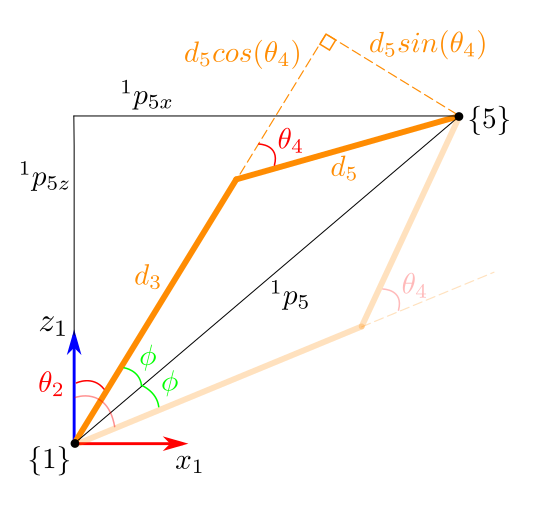
\includegraphics[width=8cm]{images/th2-4-calculation.png}\\
\caption{Calculation of angles $θ_2, θ_4$}
\label{iiwa14-solution-configurations}
\end{figure}
\end{center}

\begin{equation}
φ = acos \left( \frac{d_3^2 + \Vert{}^1p_{5}\Vert ^2 - d_5^2}{2d_3 \Vert{}^1p_{5}\Vert} \right)
\end{equation}
\begin{equation}
θ_2 = atan2 \left( \sqrt{p_x^2 + p_y^2}, {}^1p_{5z} \right) \pm φ
\end{equation}

\[ c_4 = \frac{ \Vert{}^1p_{5}\Vert ^2 - d_3^2 - d_5^2 }{2d_3d_5} \]
\begin{equation}
θ_4 = atan2 \left( \pm \sqrt{1 - c_4^2}, c_4 \right)
\end{equation}

Once $θ_1,θ_2,θ_3,θ_4$ are known, the orientation matrix of the wrist can be calculated as following
\[
R_{target} = 
\begin{bmatrix}
i_x & j_x & k_x\\
i_y & j_y & k_y\\
i_z & j_z & k_z\\
\end{bmatrix}
\]
\begin{equation}
θ_6 = atan2 \left( \pm \sqrt{1-k_y^2}, k_y \right)
\end{equation}
\[
θ_7 = atan2 \left( -j_y, i_y \right)
\]
\[
θ_5 = atan2 \left( - k_z, k_x \right)
\]

\begin{center}
\begin{figure}[!htb]
\centering
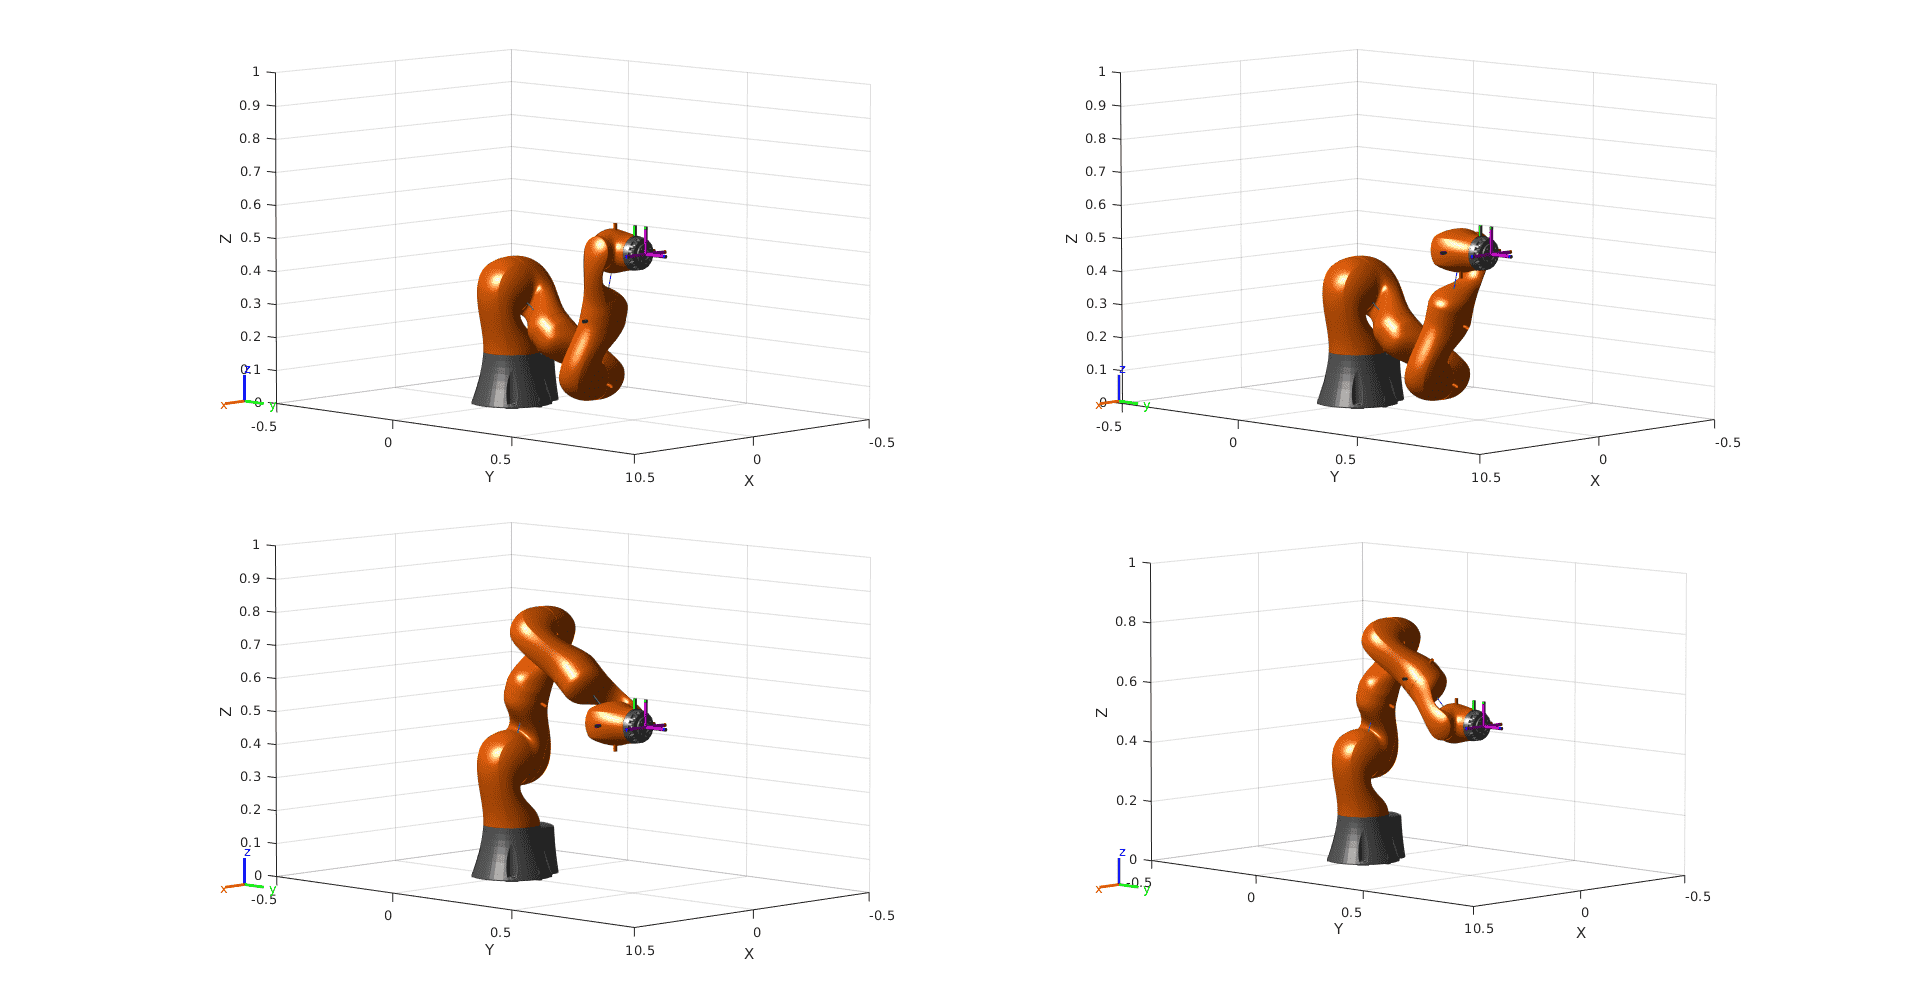
\includegraphics[width=0.8\textwidth]{images/ik-4-solutions.png}\\
\caption{The first 4 out of 8 solutions of the Inverse Kinematics problem, using the decoupling technique}
\end{figure}
\end{center}


\subsection{Solutions for 7DoF numerically}

To solve numerically for the joint angles, we use a relationship between the derivative of the spatial coordinates and the joint derivatives. These two vectors 
are related by a matrix known as the \textbf{Jacobian} and is given by the following equation

\begin{equation}
\mathbf{\dot{x}} = J( \mathbf{q} ) \mathbf{\dot{q}}
\end{equation}

where

\begin{equation}
J( \mathbf{q} ) = \begin{bmatrix}
\dfrac{\partial \mathbf{f}_1(\mathbf{q})}{\partial q_{1}} & \cdots & \dfrac{\partial \mathbf{f}_1(\mathbf{q})}{\partial q_{7}} \\
\vdots & \ddots & \vdots \\
\dfrac{\partial \mathbf{f}_6(\mathbf{q})}{\partial q_{1}} & \cdots & \dfrac{\partial \mathbf{f}_6(\mathbf{q})}{\partial q_{7}} \\
\end{bmatrix}
\end{equation}

and the functions $\mathbf{f}_i(\mathbf{q})$ are calculated using the robot's forward kinematics.

$J( \mathbf{q} )$ is non rectangular and thus non-invertible, due to the extra degree of freedom. Instead of the inverse of the Jacobian the pseudoinverse is calculated which by the 
equation
\begin{equation}
J^{\dagger} = J^\top ( J J^\top )^{-1}
\end{equation}

\begin{algorithm}[H]
\SetAlgoLined
initialize $\mathbf{q}^0 \in \mathbb{R}^{7}$ with an initial guess, given a desired position and orientation $\mathbf{x}_d \in \mathbb{R}^{6}$\;
set error $e = \mathbf{x}_d - f(\mathbf{q^i})$\;
set error tolerance $ε$ with some small value\;
\While{$e \geq ε$}{
	set $\mathbf{q}^{i+1} = \mathbf{q}^i + J^{\dagger}( \mathbf{q} )e$\;
	$i \leftarrow i + 1$\;
}
\caption{Newton-Raphson numerical method}
\end{algorithm}

If the numerical method has more than one solutions, then the method will converge to the one which is closest to the initial guess or it will not converge at all, 
if the initial error is too big. One way to get some approximate initial guesses is if we use a solution from the previous section (which solves for 6 dof) and use these 
solutions as input to this numerical method.

The numerical calculation of the inverse kinematics can also be calculated using the geometric Jacobian, given by the following equation
\[
J_v = J_v( \mathbf{q} ) = [ J_{v1}, J_{v2}, \cdots, J_{v7} ] \in \mathbb{R}^{6 \times 7}
\]
\begin{equation}
J_i = \begin{bmatrix}
{}^0\mathbf{z}_i \times ({}^0\mathbf{p}_8 - {}^0\mathbf{p}_i) \\
{}^0\mathbf{z}_i \\
\end{bmatrix}
\end{equation}


\subsection{Comparison of Inverse Kinematics Techniques}


\subsection{Constraints \& Singularity points}

\subsubsection{Workspace constraints \& Singularity points}
\begin{center}
\begin{figure}[!htb]
\centering
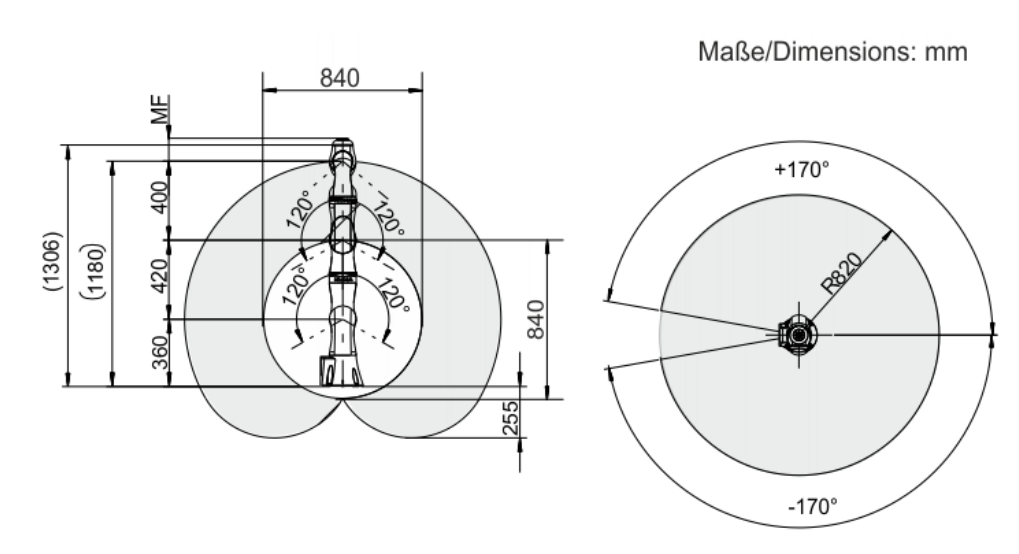
\includegraphics[width=10cm]{images/iiwa-workspace.png}\\
\caption{KUKA iiwa LBR14 workspace dimensions}
\end{figure}
\end{center}

Singularity points:
\begin{itemize}
	\item When $p_x^2 + p_y^2 = 0$ then the end-effector lies on the z-axis and $θ_1$ is not defined
	\item When $sin\left( θ_6 \right) = 0$ then the angles $θ_5, θ_7$ are not defined
\end{itemize}

\subsubsection{Remote Center of Motion constraint}
\label{rcm-subsubsection}


\subsubsection{Elbow-up constraint}
\label{section-elbow-up-constraints}

The inverse kinematic problem usually outputs 8 different solutions, all of which satisfy the same target position and orientation for the end-effector, but with different arm configurations (see figures 
\ref{iiwa14-solution-configurations} and \ref{elbow-up-vs-down}). These solutions offer more flexibility to each case, and a different solution is chosen based on the conditions (e.g. previous robot pose) and 
requirements (e.g. collision avoidance). In this thesis, there are 2 distinct use cases in terms of choosing a specific robot configuration picking the surgical tools from one table, which does not impose any constraint
and the insertion and pivoting of the surgical tool at the mounting dock, which imposes the RCM constraint (see \ref{rcm-subsubsection}) and a constraint to of collision avoidance between the robot arm and the mounting dock.
In the latter use case, in order to satisfy the collision avoidance, all path planning kinematic solutions must be in a elbow-up configuration at all times.

\begin{center}
\begin{figure}[!htb]
\centering
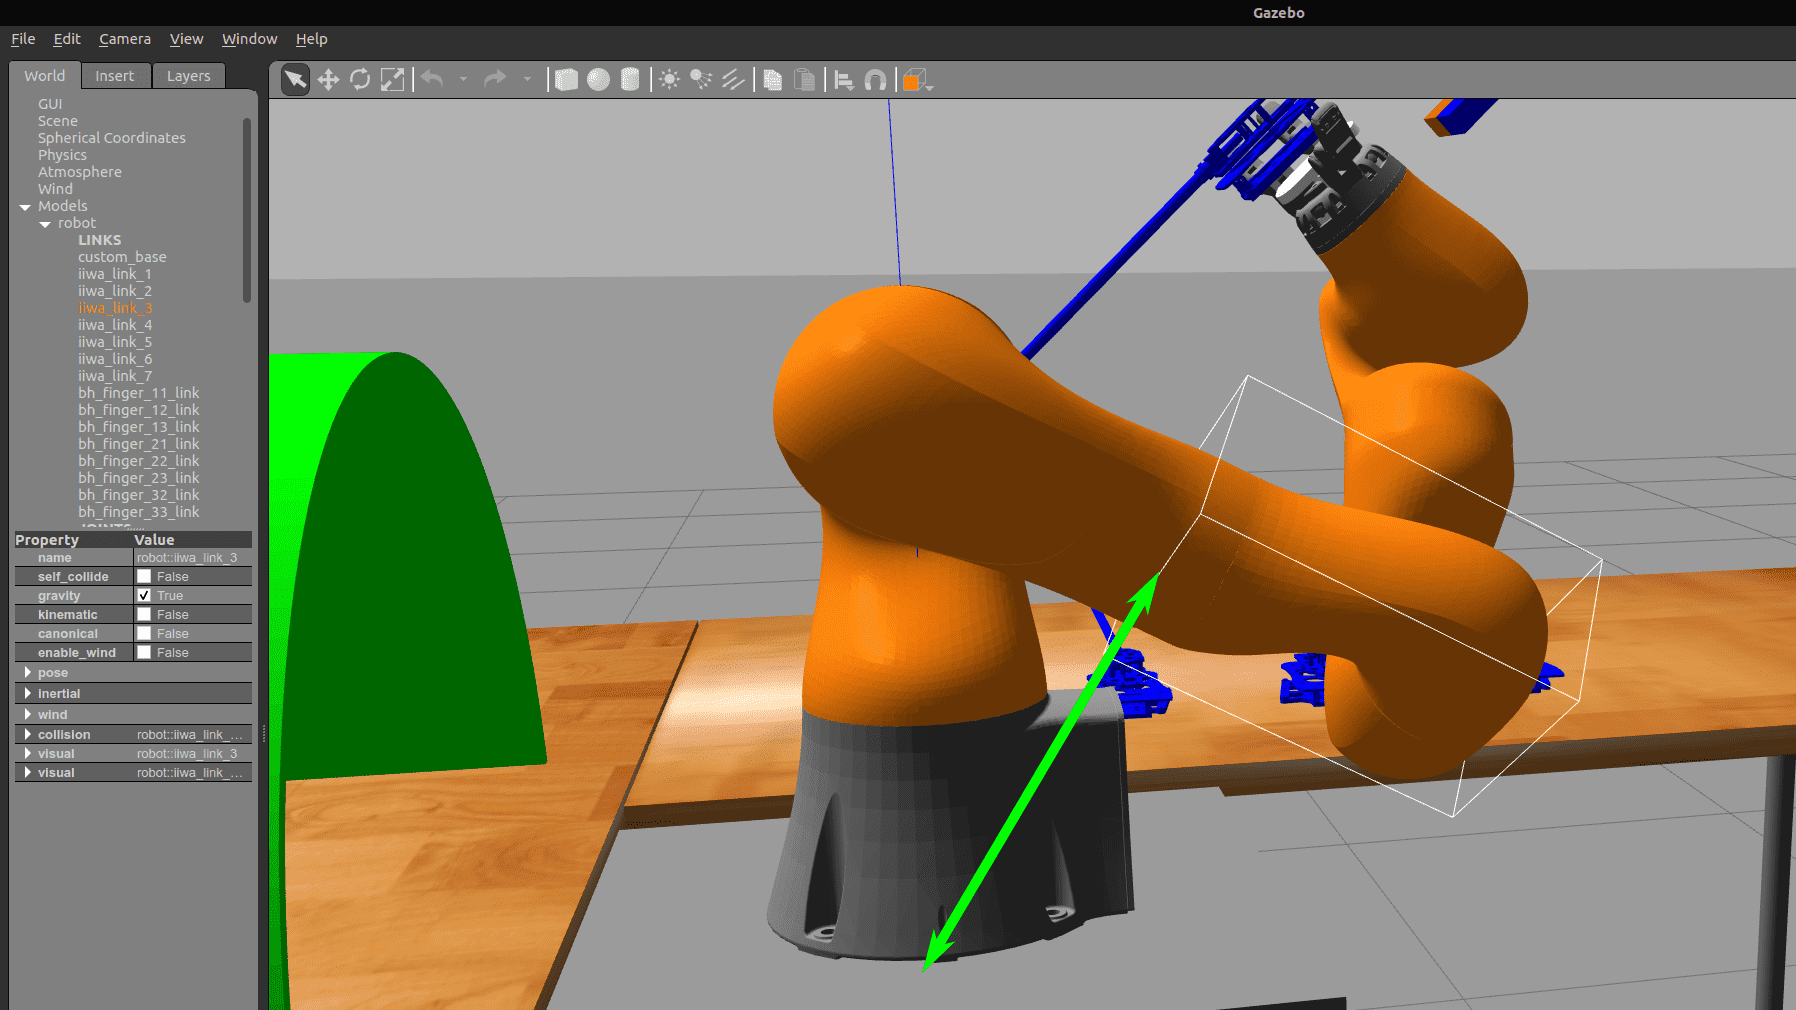
\includegraphics[width=\textwidth]{images/elbow-down.png}\\
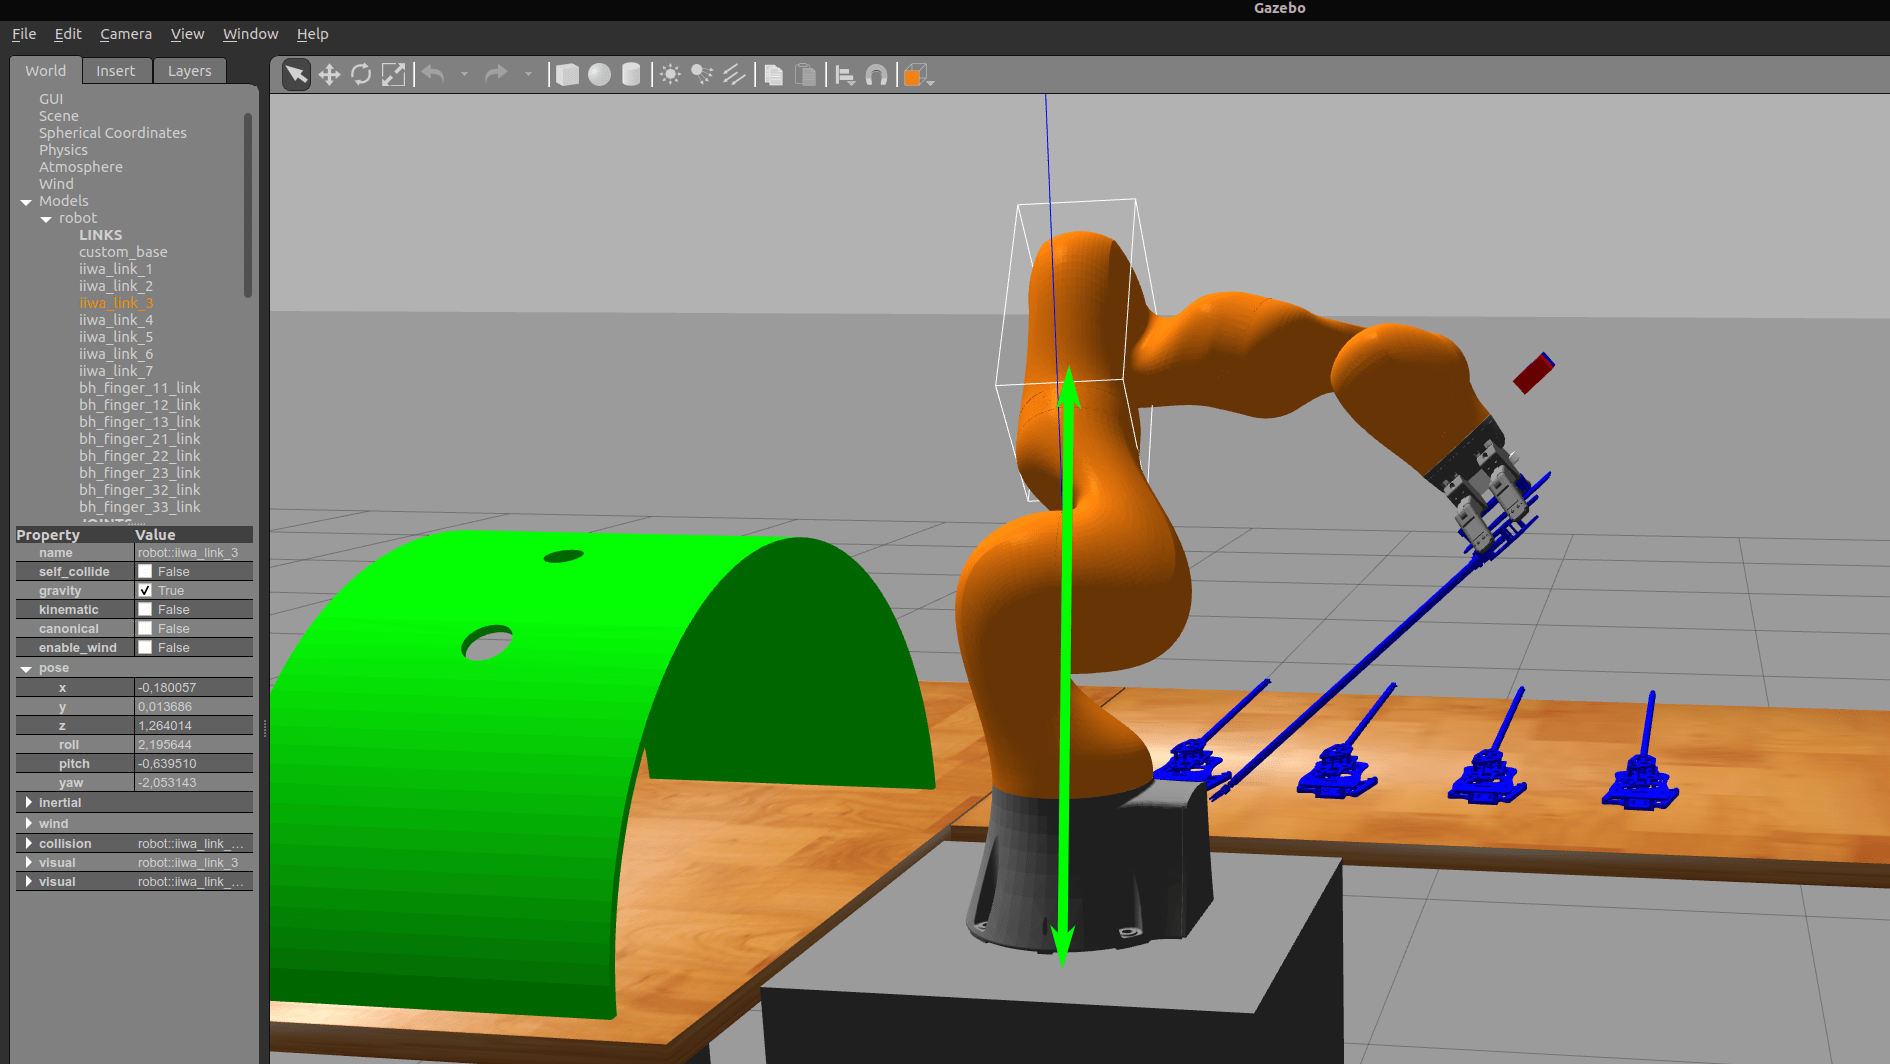
\includegraphics[width=\textwidth]{images/elbow-up.png}\\
\caption{Top: elbow-down solution, bottom: elbow-up solution}
\label{elbow-up-vs-down}
\end{figure}
\end{center}

Observing the screenshots at \ref{elbow-up-vs-down}, there are 2 ways to mathematically describe the elbow-up constraint (see figure \ref{elbow-up-constraint-geometry} below), either using distance between the robot base and 
the 3rd link or by using the relative angle of the base link and the 3rd link. From the iiwa14 specifications, the following calculations are done using $d_1 = 360mm$ and $d_3 = 420mm$.

\begin{center}
\begin{figure}[!htb]
\centering
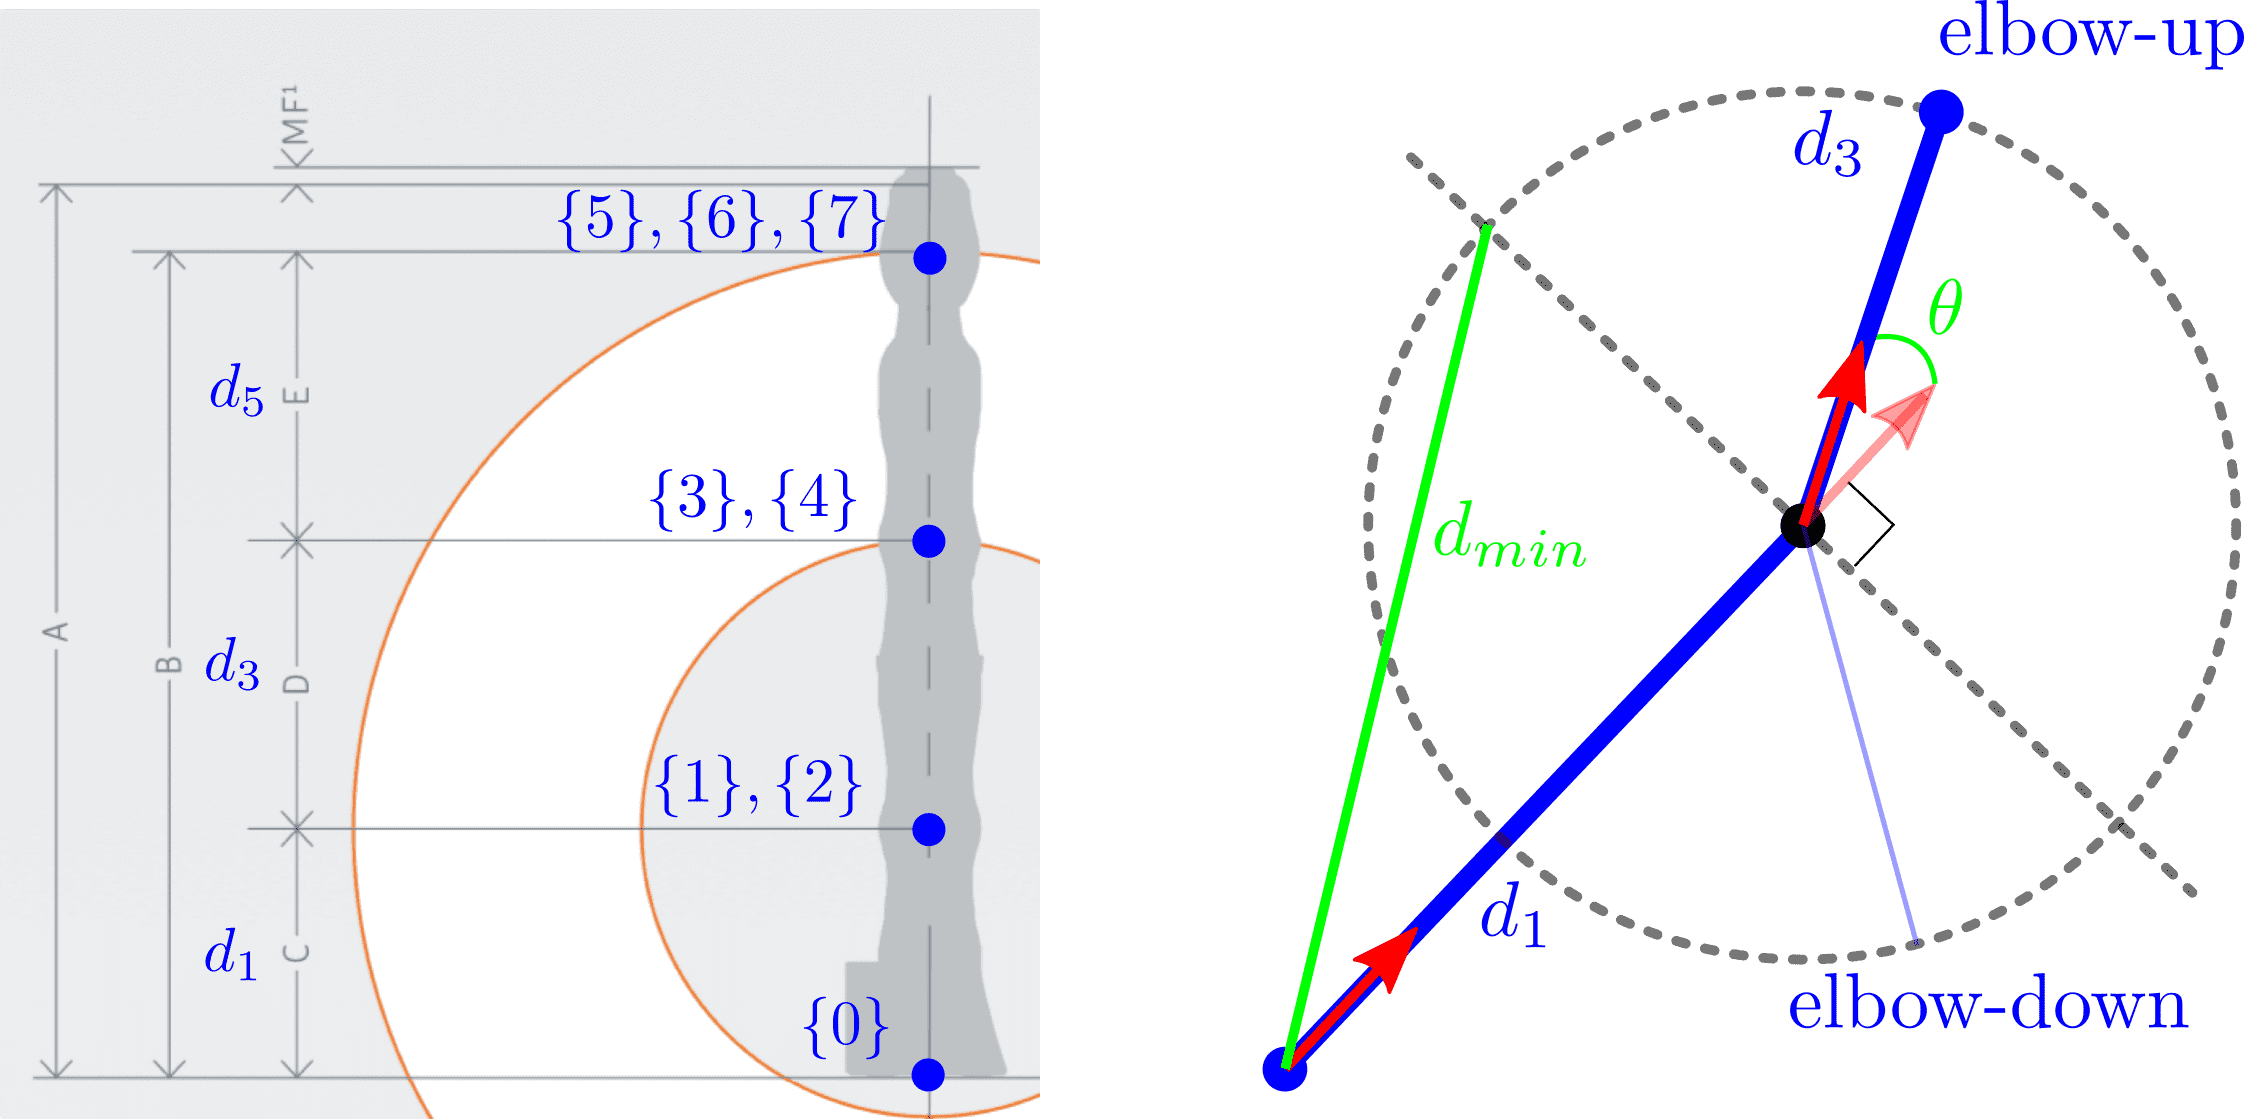
\includegraphics[width=\textwidth]{images/elbow-up-constraint-geometry.png}\\
\caption{Elbow-up constraint description with relative distance or angle between links with lengths $d_1$ and $d_3$}
\label{elbow-up-constraint-geometry}
\end{figure}
\end{center}

The distance constraint is $d_{min} \leq d \leq d_{max} $, where
\[
d_{min} = \sqrt{d_1^2 + d_3^2} = 553mm  \quad \textrm{and} \quad  d_{max} = d_1 + d_3 = 780mm
\]
The distance-based description of the elbow-up constraint is not very convenient, because it can not be easily transformed to a description that uses the robot's forward kinematic transformations and reference frames. 
For this reason, the angle-based description is more convenient because it directly describes the orientation that the 3rd reference frame must have, with respect to the reference frame of the base. Thus for each orientation 
angle (pitch, yaw, roll) the following constraint must be satisfied
\[
-\frac{\pi}{2} \leq θ \leq \frac{\pi}{2}
\]
